\subsection{Avancées et prévisions}

    \subsubsection{Cahier des charges}

    \paragraph{Répartition des tâches}
        Les tâches étaient à l'origine, réparties comme suit, mais certaines modifications ont dû y être apportées 
        à cause de certains contretemps.


        \begin{table}[!htb]
            \begin{tabular}{|l|l|l|}
            \hline
            \textbf{Tâche}                         & \textbf{Responsable}               & \textbf{Suppléant}                 \\ \hline
            \multicolumn{3}{|l|}{\cellcolor[HTML]{343434}{\color[HTML]{FFFFFF} \textbf{Carte}}}                              \\ \hline
            Création de la carte                   & \cellcolor[HTML]{9698ED}Paul       & \cellcolor[HTML]{34FF34}Renaud-Dov \\ \hline
            Création du lobby                      & \cellcolor[HTML]{34FF34}Renaud-Dov & \cellcolor[HTML]{9698ED}Paul       \\ \hline
            \multicolumn{3}{|l|}{\cellcolor[HTML]{343434}{\color[HTML]{FFFFFF} \textbf{Réseau}}}                             \\ \hline
            Implémentation du multijoueur          & \cellcolor[HTML]{34CDF9}Julien     & \cellcolor[HTML]{F8A102}Harrys     \\ \hline
            \multicolumn{3}{|l|}{\cellcolor[HTML]{343434}{\color[HTML]{FFFFFF} \textbf{IA}}}                                 \\ \hline
            Réalisation des différents types d'IA  & \cellcolor[HTML]{34FF34}Renaud-Dov & \cellcolor[HTML]{9698ED}Paul       \\ \hline
            \multicolumn{3}{|l|}{\cellcolor[HTML]{343434}{\color[HTML]{FFFFFF} \textbf{Menus}}}                              \\ \hline
            Interface                              & \cellcolor[HTML]{34CDF9}Julien     & \cellcolor[HTML]{F8A102}Harrys     \\ \hline
            HUD                                    & \cellcolor[HTML]{F8A102}Harrys     & \cellcolor[HTML]{34CDF9}Julien     \\ \hline
            \multicolumn{3}{|l|}{\cellcolor[HTML]{343434}{\color[HTML]{FFFFFF} \textbf{Game Core}}}                          \\ \hline
            Contrôle du personnage                 & \cellcolor[HTML]{34FF34}Renaud-Dov & \cellcolor[HTML]{F8A102}Harrys     \\ \hline
            Animations                             & \cellcolor[HTML]{34FF34}Renaud-Dov &                                    \\ \hline
            Objets dynamiques                      & \cellcolor[HTML]{34FF34}Renaud-Dov & \cellcolor[HTML]{F8A102}Harrys     \\ \hline
            Déroulé d'une partie                   & \cellcolor[HTML]{F8A102}Harrys     & \cellcolor[HTML]{9698ED}Paul       \\ \hline
            \multicolumn{3}{|l|}{\cellcolor[HTML]{343434}{\color[HTML]{FFFFFF} \textbf{Autre}}}                              \\ \hline
            Système de progression                 & \cellcolor[HTML]{F8A102}Harrys     &                                    \\ \hline
            Réalisation et maintenance du site Web & \cellcolor[HTML]{9698ED}Paul       & \multicolumn{1}{c|}{-}             \\ \hline
            \end{tabular}
        \end{table}
        

        \begin{table}[!htb]
            \begin{tabular}{l||lll}
                \rowcolor[HTML]{000000} 
                
                {\color[HTML]{FFFFFF} \backslashbox{\textbf{Tâche}}{\textbf{Soutenance}}} & {\color[HTML]{FFFFFF} \textbf{Soutenance 1}} & {\color[HTML]{FFFFFF} \textbf{Soutenance 2}} & {\color[HTML]{FFFFFF} \textbf{Soutenance 3}} \\
                \rowcolor[HTML]{FFFFFF} 
                \textbf{Mouvement} & 50\% & 70\% & 100\% \\
                \rowcolor[HTML]{C0C0C0}
                \textbf{Interfaces/HUD} & 40\% & 60\% & 100\% \\
                \textbf{Cartes} & 40\% & 80\% & 100\% \\
                \rowcolor[HTML]{C0C0C0} 
                \textbf{Réseau} &20\% & 50\% & 100\% \\
                \textbf{IA} & 30\% & 60\% & 100\% \\
                \rowcolor[HTML]{C0C0C0} 
                \textbf{Mécaniques de jeu} & 50\% & 70\% & 100\% \\
                \textbf{Progression} & 20\% & 60\% & 100\% \\
                \rowcolor[HTML]{C0C0C0}
                \textbf{Site internet} & 0\% & 100\% & 100\%
            \end{tabular}
        \end{table}




    \subsubsection{Première soutenance}

        \begin{table}[!hbt]
            \begin{center}
                \begin{tabular}{l|ll}
                    \rowcolor[HTML]{000000} 
                    {\color[HTML]{FFFFFF} \backslashbox{\textbf{Partie}}{\textbf{Tâche}}} & {\color[HTML]{FFFFFF} \textbf{Prévu}} & {\color[HTML]{FFFFFF} \textbf{Réalisé}} \\
                    \rowcolor[HTML]{FFFFFF} 
                    \textbf{Mouvement}                         & 50\%                                  & \cellcolor[HTML]{FFCC67}80\%         \\
                    \rowcolor[HTML]{C0C0C0} 
                    \textbf{Interface/HUD}                    & 40\%                                  & \cellcolor[HTML]{68CBD0}40\%         \\
                    \textbf{Cartes}                            & 40\%                                  & \cellcolor[HTML]{68CBD0}40\%         \\
                    \cellcolor[HTML]{C0C0C0}\textbf{Réseau}    & \cellcolor[HTML]{C0C0C0}20\%          & \cellcolor[HTML]{FFCC67}50\%         \\
                    \textbf{IA}                                & 30\%                                  & \cellcolor[HTML]{FFCC67}40\%         \\
                    \rowcolor[HTML]{C0C0C0} 
                    \textbf{Mécaniques de jeu}                 & 50\%                                  & \cellcolor[HTML]{FD6864}40\%         \\
                    \textbf{Progression}                       & 20\%                                  & \cellcolor[HTML]{FFCC67}30\%        
                    \end{tabular}
            \end{center}
            \caption{Tableau des avances et retards dans les différentes parties}
        \end{table}

    
    \subsubsection{Prévisions pour la deuxième soutenance}

        \paragraph{Map}
        Afin d'améliorer l'expérience des joueurs, nous réfléchissons actuellement à la création d'une 
        seconde map, une fois la première peaufinée.

        \paragraph{Interface}
        Sur l’interface, nous prévoyons d’intégrer la catégorie « Liste des serveurs » au menu Multijoueur. 
        Les joueurs pourront ainsi choisir librement le serveur qu’ils souhaitent rejoindre. 
        Ce menu permettrait aussi aux joueurs souhaitant s'amuser en petit comité de créer des 
        parties privées grâce à un onglet "Créer un serveur" à partir de paramètres personnalisables. 
        Il sera également possible de connaître les noms des joueurs connectés à la partie en pressant 
        la touche TAB grâce à un menu présent en jeu.

        \paragraph{Réseau}
        Nous souhaitons ajouter un chat textuel dans le lobby et au sein des parties mêmes afin d’augmenter la sociabilité et l’adversité entre les joueurs.

        \paragraph{Intelligence Artificielle}
        Pour la seconde période, notre objectif serait de pouvoir avoir une IA plus autonome et intelligente, qui n'emprunte plus forcément le chemin le plus court. 
        De plus, les joueurs peuvent actuellement bousculer les NPC qui s'arrêtent alors de marcher, mais ils ne peuvent jamais les pousser; 
        ceci sera donc à paufiner.

        \paragraph{Mécaniques de jeu}
        Nous prévoyons d'intégrer pour la deuxième soutenance des pouvoirs
        comme un écran de fumée ou encore des couteaux,
        pour rendre le jeu plus intéréssant et dynamique.\\
        Nous comptons également implémenter le script de choix de la cible.
        Même si celui-ci a été réalisé il n'est pas encore utilisé en jeu.
        Il faudra principalement donner un sens à l'attribution des cibles,
        sous la forme de points octroyés au joueur.

        \paragraph{Autres}
        Pour tester le multijoueur avec des invités, nous avons réalisé 
        un début de launcher qui télécharge les dernières mises à jour et les installe.
        Nous aimerions continuer à le développer pour avoir un lanceur
        qui se mette à jour automatiquement sans à avoir à le réinstaller.


    \subsubsection{Deuxième soutenance}

        \paragraph{Avancées}
        \begin{table}[!hbt]
            \begin{center}
                \begin{tabular}{l|ll}
                    \rowcolor[HTML]{000000} 
                    {\color[HTML]{FFFFFF} \backslashbox{\textbf{Partie}}{\textbf{Tâche}}} & {\color[HTML]{FFFFFF} \textbf{Prévu}} & {\color[HTML]{FFFFFF} \textbf{Réalisé}} \\
                    \rowcolor[HTML]{FFFFFF} 
                    \textbf{Mouvement}                         & 70\%                                  & \cellcolor[HTML]{31943b}70\%         \\
                    \rowcolor[HTML]{C0C0C0} 
                    \textbf{Interface/HUD}                     & 60\%                                  & \cellcolor[HTML]{ed5113}50\%         \\
                    \textbf{Cartes}                            & 80\%                                  & \cellcolor[HTML]{31943b}90\%         \\
                    \rowcolor[HTML]{C0C0C0}
                    \textbf{Réseau}    						   & 50\%          						   & \cellcolor[HTML]{31d12a}70\%         \\
                    \textbf{IA}                                & 60\%                                  & \cellcolor[HTML]{31d12a}80\%         \\
                    \rowcolor[HTML]{C0C0C0} 
                    \textbf{Mécaniques de jeu}                 & 70\%                                  & \cellcolor[HTML]{31d12a}80\%         \\
                    \textbf{Progression}                       & 60\%                                  & \cellcolor[HTML]{ed5113}50\%        
                    \end{tabular}
            \end{center}
            \caption{Tableau des avancées et prévisions}
        \end{table}


    \subsubsection{Prévisions pour la troisième soutenance}

        Le jeu est à présent dans un état "jouable". Cependant, il faut encore implémenter de nombreux systèmes pour finaliser notre vision pour le projet.

        \paragraph{Multiplayer}
        Certains systèmes ont été créés, comme les finishers ou les pouvoirs, mais n'ont pas encore été 
        implémentés en multijoueur. L'objectif pour la prochaine soutenance sera donc d'intégrer les mécaniques 
        de jeu qui ne l'ont pas encore été au réseau Photon pour permettre au joueurs d'y accéder. De plus, le 
        travail continue sur la synchronisation ie. des personnages joueurs et non-joueurs, notamment il est 
        question d'optimisation pour le mouvement des IA qui génère encore une utilisation de bande passante importante. 
        Il serait intéressant de tenter l'utilisation d'une méthode de compression pour les vecteurs afin de diminuer 
        la quantité d'information envoyée.

        \paragraph{Progression}
        Bien qu'un système d' expérience et de niveau ait été implémenté, celui-ci n'a pour l'instant pour 
        l'instant pas d'utilité. Mais de nombreuses opportunités de progression se sont ouvertes, 
        notamment grâce au travail de Dov. Par exemple, nous comptons permettre le débloquage des 
        finishers grâce à ce système de progression. Nous pourrons également modifier le système actuel 
        de customisation de personnage et restreindre l'utilisation de certaines options d'apparence à un certain niveau.

        \paragraph{Tableau des scores}
        Le scoreboard reste très simple et manque d’informations. Nous souhaiterions donner au tableau des scores un affichage plus épuré et plus simple. Une mise en tableau des différentes informations permettrait d’éviter au texte de dépasser les bordures du canvas. Elle facilitera grandement l’ajout, la suppression ou la modification d’une valeur ou d’un joueur pendant la partie ainsi que l’alignement des valeurs appartenant a la même categorie. 
        Cette nouvelle version du tableau comprendrait l'affichage des points, du nombre de fois où le joueur est mort, le nombre de fois où il a tué un joueur, le nombre de fois où il a tué une IA et son PING avec le serveur. Ce formatage sous forme de tabeau permet aussi de faire une sauvegarde rapide et temporaire du tableau dans les fichiers du jeu. Il serait ainsi beaucoup plus simple pour le logiciel d'y accéder et de l'éditer.
        
        \begin{figure}[hbt!]
        \centering
            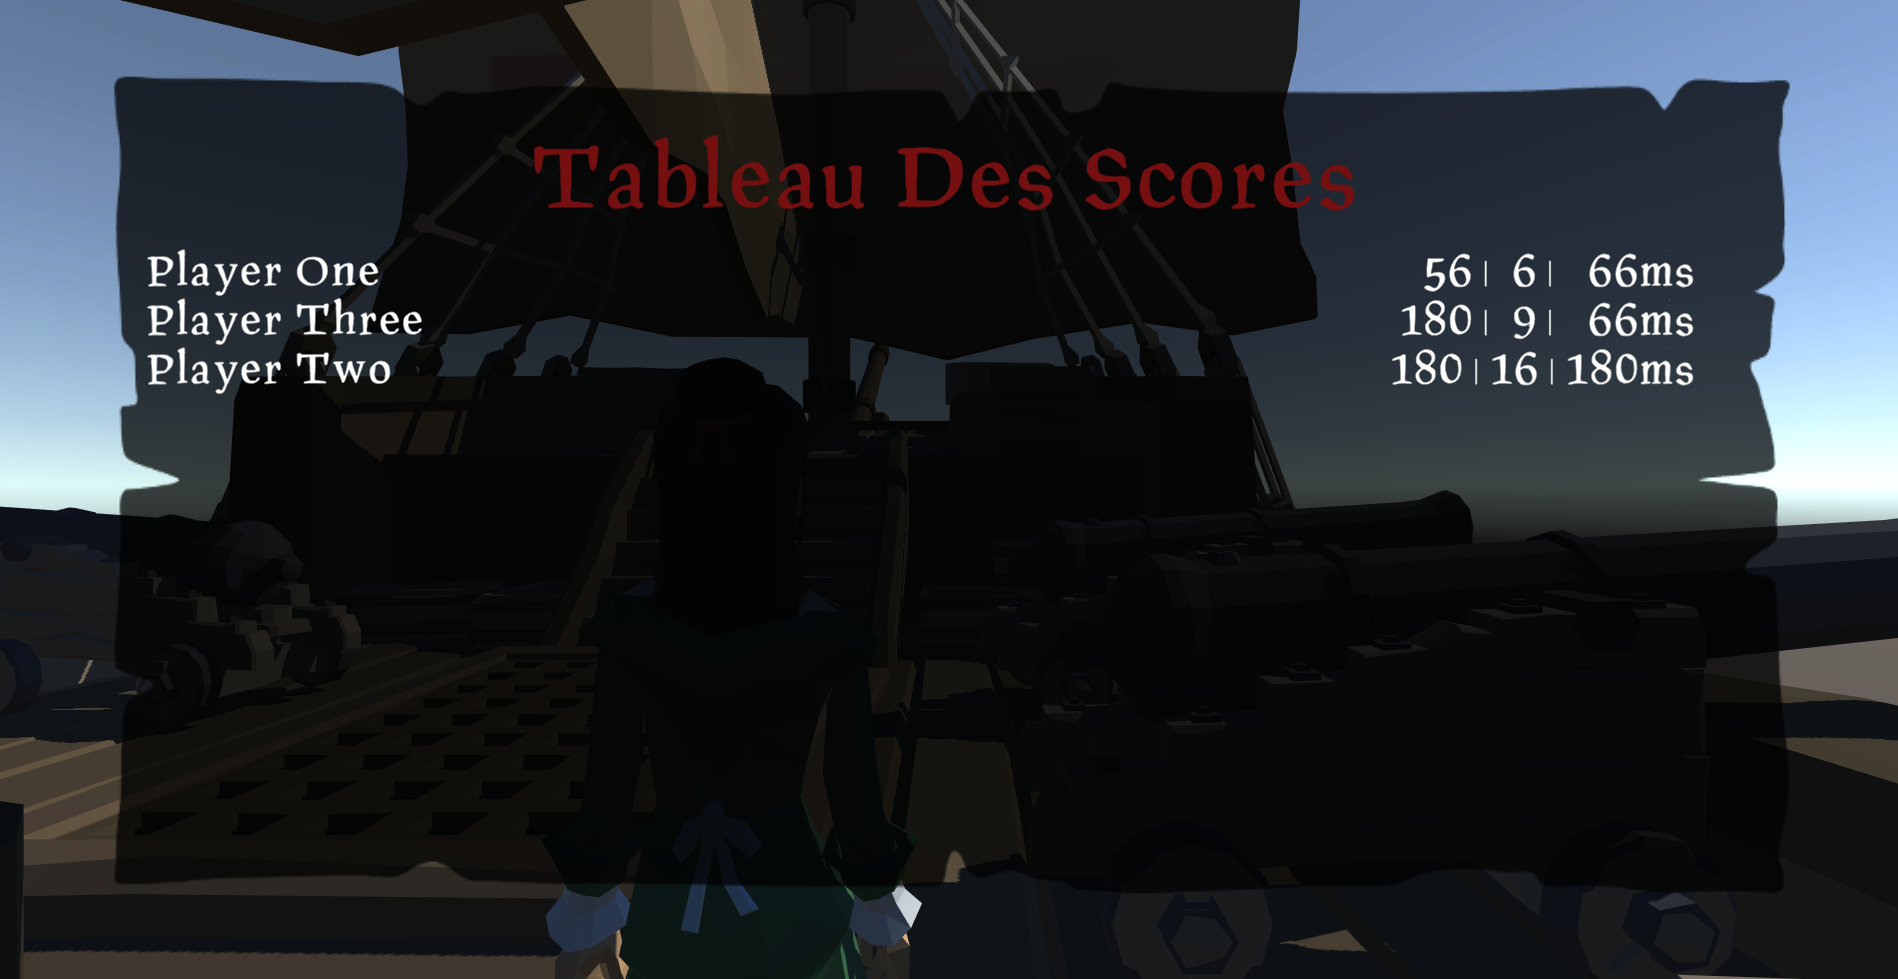
\includegraphics[scale=0.29]{img/newscoreboard.PNG}
            \caption{Seconde version du tableau des scores}
        \end{figure}


        \paragraph{HUD}
        Certaines informations sont essentielles pour le joueur. Elles lui permettent de savoir en cours de partie et à n'importe quel moment quel pouvoir il peut utiliser, combien de temps il lui reste avant de pouvoir l'utiliser (si son pouvoir necessite un temps de rechargement), la cible qui lui a été désigné par le jeu ou encore de pouvoir lire le chat général en direct.
        
        \begin{figure}[hbt!]
                \centering
                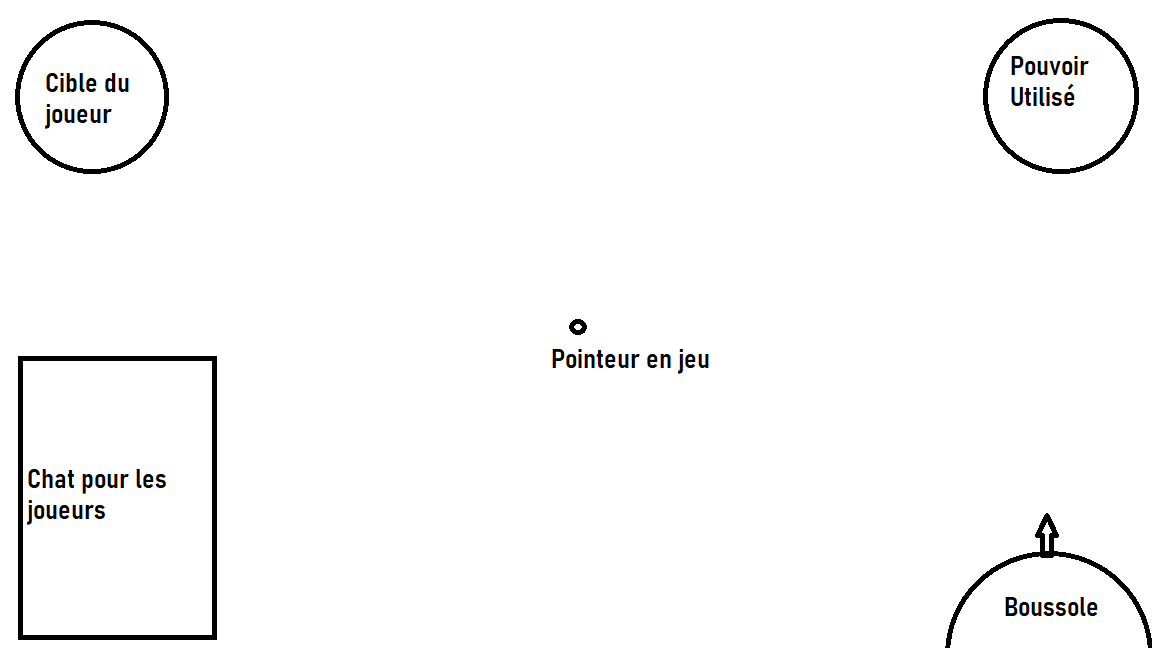
\includegraphics[scale=0.3]{img/schem_hud.png}
                \caption{Schéma du futur HUD}
        \end{figure}
        

        \paragraph{Carte}

        Pour la prochaine soutenance, l'objectif est d'avoir une map terminée dans les moindres 
        détails. Comme cet objectif semble raisonnable, un seconde carte est aussi une possibilité 
        envisagée pour l'ultime soutenance.

    
    \subsection{Troisième soutenance}

        % à compléter